\documentclass[journal]{IEEEtran}

\usepackage{cite}
\usepackage{amsmath,amssymb,amsfonts}
\usepackage{graphicx}
\usepackage{booktabs}
\usepackage{tabularx}
\usepackage{array}
\usepackage{multirow}
\usepackage{url}
\usepackage{xspace}
\usepackage{xcolor}
\usepackage{tikz}
\usetikzlibrary{arrows.meta,positioning,fit,shapes.geometric,calc}

\graphicspath{{../../ICPP-demo/}{../../../results/intel/wordcount_sweep/figures/}{../../../results/intel/}}

\newcommand{\briskstate}{BriskState\xspace}
\newcommand{\system}{\briskstate}
\newcolumntype{L}[1]{>{\raggedright\arraybackslash}p{#1}}
\newcolumntype{C}[1]{>{\centering\arraybackslash}p{#1}}
\newcolumntype{Y}{>{\raggedright\arraybackslash}X}

\begin{document}

\title{\briskstate: A Cache-Aware State Backend for Apache Flink}

\author{Anonymous Authors}

\maketitle

\begin{abstract}
State access dominates the cost of many stream-processing pipelines once working sets outgrow cache capacity and garbage-collection overhead becomes visible at runtime. This paper presents \system, a cache-aware keyed state backend for Apache Flink that reorganizes state by key-group and namespace, uses compact Swiss-table-inspired layouts for hot paths, and integrates copy-on-write snapshotting with Flink's checkpoint protocol. \system combines a Java control layer, a lightweight keyed state store, specialized primitive-key tables, and a native execution path for off-heap state management. We evaluate the design with correctness tests, operator-level state benchmarks, WordCount grid sweeps, end-to-end NexMark queries, and microarchitectural profiling. Across 184 tests, \system preserves Flink-compatible semantics and checkpoint behavior. On an Intel reference platform, \system improves WordCount throughput on all 36 scanned configurations, with a 1.270$\times$ average and 1.414$\times$ peak speedup over the heap baseline; it improves 13 of 14 state-benchmark operations, including +132\% for list iteration and +110\% for map insertion; and it shortens state-intensive NexMark queries substantially under tight memory budgets while eliminating several stuck configurations. VTune results show that the same design reduces Memory Bound from 48.1\% to 15.3\% and DRAM Bound from 30.8\% to 2.2\%. The results show that layout-aware keyed state organization can materially improve both throughput and runtime stability in Flink workloads.
\end{abstract}

\begin{IEEEkeywords}
Apache Flink, stream processing, state backend, memory locality, snapshotting, Swiss tables
\end{IEEEkeywords}

\section{Introduction}

Stateful stream processing systems execute user logic over continuously evolving keyed state. In Apache Flink, this path is exercised by point updates, aggregations, joins, timers, windows, and checkpointing logic, so state management often dominates end-to-end performance once working sets exceed cache capacity or heap pressure increases \cite{carbone2015flink,carbone2017statemanagement}. Under these conditions, latency and throughput are controlled less by arithmetic throughput and more by the structure of the state-access path: pointer indirection, object layout, probe locality, snapshot capture, and the interaction between state growth and runtime memory management.

The default choices available to many Flink deployments present a familiar trade-off. Heap-resident state can deliver low software overhead while memory pressure remains moderate, but it becomes sensitive to object layout and garbage collection as state grows. Embedded persistent stores such as RocksDB bound heap growth and provide robustness, but they trade low-latency in-memory access for additional serialization, compaction, and storage-layer overhead \cite{rocksdb}. This leaves an open design space for backends that remain fully integrated with Flink's keyed-state abstractions and checkpoint protocol while organizing state more explicitly for locality.

This paper studies that design space through \system, a cache-aware keyed state backend that partitions state by key-group and namespace, stores entries in compact Swiss-table-inspired structures, and integrates snapshotting via copy-on-write (CoW) views and batched asynchronous serialization. The implementation builds on a Java control layer and a Flink-compatible keyed backend, while exposing specialized fast paths for primitive keys and an optional native execution path for off-heap state management. The central claim is not that one hash table alone determines system performance, but rather that state layout, snapshot capture, and keyed partitioning jointly shape the runtime behavior of stream-processing jobs.

The paper makes the following contributions.
\begin{itemize}
\item It presents the design of \system as a Flink-compatible keyed state backend that reorganizes the state path around key-group partitioning, namespace-aware routing, compact Swiss-table-style storage, and CoW snapshotting.
\item It describes an implementation that combines a lightweight keyed state store, specialized primitive-key state tables, asynchronous checkpoint serialization, and a native execution path while preserving the semantics of Flink's state APIs and savepoint/checkpoint formats.
\item It provides a multi-level evaluation that spans correctness, operator-level state benchmarks, workload-level microbenchmarks, end-to-end NexMark queries, and microarchitectural profiling on Intel and Kunpeng platforms.
\item It shows that layout-aware state organization can improve both throughput and robustness: on Intel, \system improves all 36 WordCount scan points, improves 13 of 14 operator-level benchmark operations, reduces pipeline memory stalls substantially, and removes several stuck NexMark configurations under tight memory budgets.
\end{itemize}

\section{Background and Motivation}

Modern stateful dataflow systems such as MillWheel, Naiad, Flink, Structured Streaming, and the Dataflow model define execution semantics for continuous queries, event time, and out-of-order processing, but they generally abstract away the physical state layout that ultimately determines runtime cost \cite{akidau2013millwheel,murray2013naiad,carbone2015flink,akidau2015dataflow,armbrust2018structured}. This abstraction is necessary for usability, but it can hide the source of performance instability when keyed state grows large enough that backend behavior becomes visible above operator logic.

Within Flink, keyed state is partitioned by key-group for scalability and checkpointing. This organization preserves determinism and enables redistribution, but each state access still depends on how keys, namespaces, and values are laid out inside the backend. Existing work on Flink state management and migration has focused on consistency, operational continuity, and reconfiguration cost rather than on exposing or optimizing memory-locality effects inside the backend itself \cite{carbone2017statemanagement,hoffman2019megaphone}. Meanwhile, recent storage and hash-table systems show that compact metadata, low-indirection probing, and careful update paths can change access cost materially \cite{chandramouli2018faster,abseil2018swisstable}.

The motivation for \system comes from three observations drawn from the repository's benchmark and delivery artifacts.
\begin{enumerate}
\item Heap-resident keyed state remains competitive while memory budgets are generous, but under tight budgets, state-intensive workloads degrade sharply because backend behavior interacts with GC and object layout.
\item Operator-level microbenchmarks isolate a repeated pattern: lookup, update, iterate, and remove operations become noticeably cheaper when key and metadata layout are made compact and regular.
\item Checkpoint cost is not only a serialization problem. The way state is captured for checkpointing affects the cost of subsequent writes, the shape of memory traffic, and the stability of job execution after snapshot boundaries.
\end{enumerate}

These observations suggest that a keyed state backend should be designed as a systems component, not merely as a logical map hidden behind an API. The rest of the paper follows that perspective.

\section{System Overview}

\system is implemented as a Flink keyed state backend with three major subsystems: a Java control plane that integrates with Flink runtime interfaces, a keyed state store that partitions state by key-group and namespace, and a snapshot subsystem that captures immutable views for asynchronous checkpoint serialization. Figure~\ref{fig:overview} summarizes the organization.

\begin{figure}[t]
\centering
\resizebox{\columnwidth}{!}{%
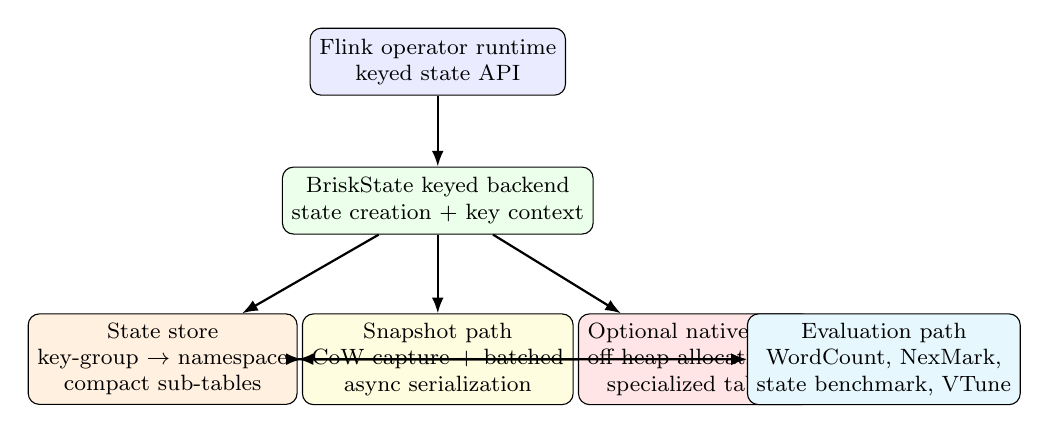
\begin{tikzpicture}[
    font=\footnotesize,
    box/.style={draw, rounded corners, align=center, minimum width=2.5cm, minimum height=0.85cm},
    small/.style={draw, rounded corners, align=center, minimum width=2.2cm, minimum height=0.72cm},
    arrow/.style={-{Latex[length=2mm]}, thick}
  ]
  \node[box, fill=blue!8] (flink) {Flink operator runtime\\keyed state API};
  \node[box, fill=green!8, below=0.9cm of flink] (backend) {\system keyed backend\\state creation + key context};
  \node[small, fill=orange!12, below left=1.0cm and -0.2cm of backend] (store) {State store\\key-group $\rightarrow$ namespace\\compact sub-tables};
  \node[small, fill=yellow!12, below=1.0cm of backend] (snap) {Snapshot path\\CoW capture + batched\\async serialization};
  \node[small, fill=red!10, below right=1.0cm and -0.2cm of backend] (native) {Optional native path\\off-heap allocation +\\specialized tables};
  \node[small, fill=cyan!10, right=2.2cm of snap] (metrics) {Evaluation path\\WordCount, NexMark,\\state benchmark, VTune};

  \draw[arrow] (flink) -- (backend);
  \draw[arrow] (backend) -- (store);
  \draw[arrow] (backend) -- (snap);
  \draw[arrow] (backend) -- (native);
  \draw[arrow] (store) -- (snap);
  \draw[arrow] (native) -- (store);
  \draw[arrow] (store) -- (metrics);
  \draw[arrow] (snap) -- (metrics);
\end{tikzpicture}%
}
\caption{High-level organization of \system. The backend is integrated with Flink keyed state APIs, while the internal path is organized around compact state storage, CoW snapshotting, and optional native acceleration.}
\label{fig:overview}
\end{figure}

At the API boundary, \system implements Flink-compatible keyed state abstractions for ValueState, ListState, MapState, ReducingState, and AggregatingState. Each abstraction uses the current key and key-group index from the keyed backend and delegates storage to a shared state-store layer. This organization avoids state-specific reinvention of routing logic and makes key-group partitioning explicit throughout the implementation.

The keyed state store is the core logical abstraction. For each registered state, it manages a collection of sub-tables indexed first by key-group and then by namespace. The special case of a void namespace, common in keyed operators such as simple per-key aggregates, is optimized separately: instead of a map from namespace to table, each key-group directly owns one table. This removes a layer of indirection on the hot path and reduces per-access routing overhead. General namespaces use a hash map per key-group so that different namespaces remain isolated and can be removed independently once empty.

The snapshot subsystem mirrors Flink's synchronous/asynchronous checkpoint split. The synchronous phase captures immutable state views with minimal blocking through CoW markers. The asynchronous phase serializes these views in batches so that data leaves the process through larger contiguous buffers rather than fine-grained entry writes. This split is central to the system because it allows the backend to reduce checkpoint interference on the main processing path without abandoning Flink's checkpoint model.

Table~\ref{tab:components} lists the major implementation surfaces that recur throughout the codebase and delivery artifacts. The table is useful because the backend is not a single data structure; it is an interaction between Flink integration, state routing, memory layout, and snapshot management.

\begin{table}[t]
\caption{Major \system components and responsibilities.}
\label{tab:components}
\centering
\small
\begin{tabularx}{\columnwidth}{L{2.4cm}Y}
\toprule
Component & Responsibility \\
\midrule
Keyed backend & Integrates with Flink keyed-state APIs, tracks current key and key-group context, creates state objects \\
State store & Organizes state as key-group $\rightarrow$ namespace $\rightarrow$ compact sub-table and manages table lifecycle \\
Swiss-style table & Executes lookup, insert, remove, grow, and rehash on compact control/payload arrays \\
Snapshot layer & Captures immutable CoW views and serializes them asynchronously with batched buffers \\
Native engine & Provides an off-heap execution path with JNI bridging and specialized storage for low-level control \\
\bottomrule
\end{tabularx}
\end{table}

Two design principles guide the remainder of the implementation. First, routing decisions should happen before object dereferences whenever possible; this is why key-group and namespace partitioning are performed above the physical table layer. Second, snapshot mechanics should preserve the compact in-memory path rather than forcing the online data structure into a serialization-friendly shape. These principles explain why \system prefers explicit table ownership, eager empty-namespace cleanup, and CoW views over general-purpose object graphs.

\section{State Organization and Access Path}

This section describes how \system organizes keyed state and why the resulting access path differs from conventional heap-resident structures.

\subsection{Key-Group and Namespace Partitioning}

Flink routes keyed state through key-groups, which already provide a natural granularity for scalability, checkpointing, and reconfiguration. \system makes key-groups the first-class storage partition. For a state instance $S$, the logical mapping is:
\begin{equation}
S : \texttt{key-group} \rightarrow \texttt{namespace} \rightarrow \texttt{sub-table}.
\end{equation}

The design has two benefits. First, it preserves a direct correspondence between runtime reconfiguration units and storage units. Second, it bounds the working set of each access to a smaller table, which improves probe locality and reduces interference across unrelated namespaces.

For void namespaces, the mapping simplifies to one sub-table per key-group. This fast path eliminates the namespace map entirely. For general namespaces, each key-group owns a namespace map whose values are sub-tables. Empty namespaces are removed eagerly after clears, which matters in window-heavy workloads where namespace churn is significant.

\subsection{Swiss-Table-Inspired Layout}

Each sub-table follows a compact layout inspired by Swiss tables. The design stores one control byte per slot in a contiguous control array and stores payloads in an interleaved array-of-structures (AoS) layout, where slot $i$ maps to the pair $(\texttt{entries}[2i], \texttt{entries}[2i+1])$ for key and value. The hash is split into a probe-dispatch component and a compact in-slot tag:
\begin{equation}
H_1 = \texttt{hash} \gg 7, \quad H_2 = \texttt{hash} \&\; 0x7F.
\end{equation}

The control byte stores either a special marker (empty or deleted) or the 7-bit $H_2$ fragment. During probing, \system loads groups of control bytes and compares them against a repeated pattern, enabling SWAR-style matching across several candidate slots at once. In the Java implementation, the default group size is eight control bytes, which matches a 64-bit load and offers a low-overhead compromise between metadata compactness and parallel candidate filtering.

This organization differs from a conventional chain of heap objects in two ways. First, metadata is separated from payload but remains densely packed, so many probe decisions are made before dereferencing keys or values. Second, the AoS payload layout keeps keys and values adjacent once the candidate slot is known, reducing the number of cache lines touched per successful access.

Figure~\ref{fig:layout} illustrates the resulting layout. The important point is not the exact byte encoding but the relative placement of routing metadata, control bytes, and payload arrays. The backend first narrows the search to one key-group and one namespace-specific sub-table, then probes compact control bytes, and only then touches the actual key/value payload.

\begin{figure}[t]
\centering
\resizebox{\columnwidth}{!}{%
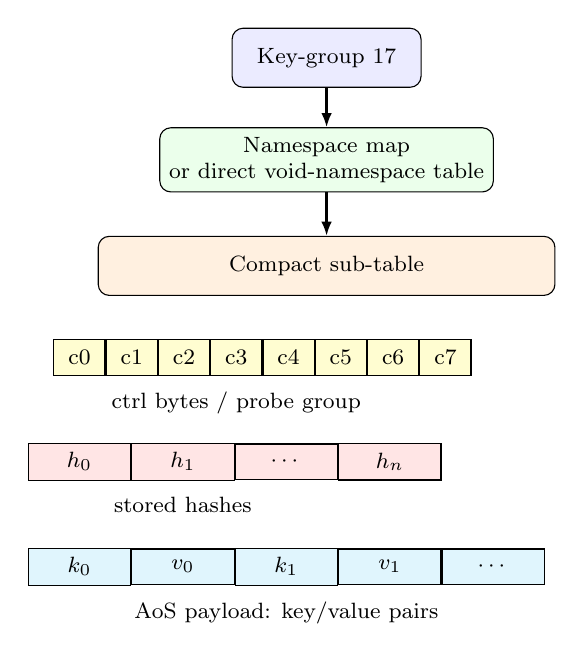
\begin{tikzpicture}[
    font=\footnotesize,
    outer/.style={draw, rounded corners, align=center, minimum height=0.75cm},
    slot/.style={draw, minimum width=0.65cm, minimum height=0.45cm, align=center},
    arrow/.style={-{Latex[length=1.8mm]}, thick}
  ]
  \node[outer, fill=blue!8, minimum width=2.4cm] (kg) {Key-group 17};
  \node[outer, fill=green!8, below=0.5cm of kg, minimum width=2.8cm] (ns) {Namespace map\\or direct void-namespace table};
  \node[outer, fill=orange!12, below=0.55cm of ns, minimum width=5.8cm] (table) {Compact sub-table};

  \node[slot, fill=yellow!18, below left=0.55cm and -0.1cm of table] (c1) {c0};
  \node[slot, fill=yellow!18, right=0cm of c1] (c2) {c1};
  \node[slot, fill=yellow!18, right=0cm of c2] (c3) {c2};
  \node[slot, fill=yellow!18, right=0cm of c3] (c4) {c3};
  \node[slot, fill=yellow!18, right=0cm of c4] (c5) {c4};
  \node[slot, fill=yellow!18, right=0cm of c5] (c6) {c5};
  \node[slot, fill=yellow!18, right=0cm of c6] (c7) {c6};
  \node[slot, fill=yellow!18, right=0cm of c7] (c8) {c7};
  \node[below=0.08cm of c4] {ctrl bytes / probe group};

  \node[slot, fill=red!10, below=0.85cm of c1, minimum width=1.3cm] (h1) {$h_0$};
  \node[slot, fill=red!10, right=0cm of h1, minimum width=1.3cm] (h2) {$h_1$};
  \node[slot, fill=red!10, right=0cm of h2, minimum width=1.3cm] (h3) {$\cdots$};
  \node[slot, fill=red!10, right=0cm of h3, minimum width=1.3cm] (h4) {$h_n$};
  \node[below=0.08cm of h2] {stored hashes};

  \node[slot, fill=cyan!12, below=0.85cm of h1, minimum width=1.3cm] (e1) {$k_0$};
  \node[slot, fill=cyan!12, right=0cm of e1, minimum width=1.3cm] (e2) {$v_0$};
  \node[slot, fill=cyan!12, right=0cm of e2, minimum width=1.3cm] (e3) {$k_1$};
  \node[slot, fill=cyan!12, right=0cm of e3, minimum width=1.3cm] (e4) {$v_1$};
  \node[slot, fill=cyan!12, right=0cm of e4, minimum width=1.3cm] (e5) {$\cdots$};
  \node[below=0.08cm of e3] {AoS payload: key/value pairs};

  \draw[arrow] (kg) -- (ns);
  \draw[arrow] (ns) -- (table);
\end{tikzpicture}%
}
\caption{Logical-to-physical organization of one \system sub-table. Routing first narrows the access to a key-group and namespace-specific table; probing then operates over compact control bytes before the key/value payload is touched.}
\label{fig:layout}
\end{figure}

\subsection{Specialized Primitive-Key Tables}

Generic object-key tables must rely on serializer output or object equality and incur boxing overhead when keys are primitive in logical form. \system therefore includes specialized tables for integer and long keys. These variants use primitive comparisons directly and can organize groups more compactly than generic object storage. A long-key group, for example, can be represented as one control word followed by a small block of keys, which reduces pointer chasing and shortens the distance between control metadata and payload.

The effect is visible most clearly in repeated update and lookup loops. In the Intel operator-level benchmark, the backend improves map insertion by 110\%, map lookup by 91\%, and value insertion by 87\%, consistent with a design whose main benefits come from shorter probe paths and reduced metadata overhead rather than from algorithmic changes at the operator level.

\subsection{State API Implementations}

The state-specific classes remain intentionally thin. ValueState maps directly to point read/update/remove operations over the state store. ListState and MapState add iteration and merge-like behaviors but still reuse the same key-group and namespace routing substrate. The keyed backend provides the current key and key-group index, so state classes can avoid redundant lookups or wrapper allocations on the hot path.

This is a design decision rather than a coding convenience. If routing, serializer interaction, and state-specific behavior are split across many layers, the state path becomes harder to reason about and optimize. \system therefore keeps state implementations close to the storage substrate and uses specialization only when it directly removes hot-path overhead.

\subsection{State-Specific Fast Paths}

The delivery design documents describe this principle more concretely as precomputed strategy selection for common key, namespace, and value combinations. The practical idea is simple: once a state descriptor is known, the backend can often choose a shorter path than a fully generic serializer-mediated route.

\begin{table}[t]
\caption{State abstractions and representative fast paths in \system.}
\label{tab:statefast}
\centering
\small
\begin{tabularx}{\columnwidth}{L{1.8cm}Y}
\toprule
State & Representative optimization \\
\midrule
ValueState & Direct point read/update/remove; primitive values prefer compact serializer paths and short key routing \\
ListState & Append and whole-list update reuse compact storage; long-element paths reduce per-element overhead \\
MapState & Typed inner-map access supports per-entry get/put/remove instead of always materializing opaque blobs \\
ReducingState & Reuses keyed routing while keeping accumulator updates close to the storage layer \\
AggregatingState & Uses the same keyed substrate with serializer-aware accumulator handling \\
\bottomrule
\end{tabularx}
\end{table}

Three implications follow. First, ValueState remains the cleanest place to observe the benefits of layout and routing because its logic is so short. Second, ListState and MapState gain from specialization not only through lookup speed but also through avoiding unnecessary whole-container materialization. Third, a single backend can expose different bottlenecks for different abstractions; this helps explain why the operator-level benchmark gains are not identical across all operations.

\section{Snapshotting and Recovery}

Checkpoint and savepoint support are mandatory for any Flink-compatible backend. \system implements these functions without abandoning the compact in-memory layout described above.

\subsection{CoW Snapshot Capture}

The synchronous checkpoint phase prepares immutable state views. Instead of serializing data immediately, the backend marks participating sub-tables as snapshotted and returns lightweight snapshot objects that retain references to the current control and payload arrays. In effect, synchronous capture is reduced to metadata preparation and reference capture.

This design makes snapshot cost proportional to the number of participating tables rather than to the volume of state. The trade-off is that the first post-snapshot mutation to a captured table may trigger a lazy clone. This is the correct trade for Flink-style workloads in which checkpoints occur periodically but most tables are not mutated immediately after every checkpoint boundary.

\subsection{Asynchronous Serialization}

The asynchronous phase consumes the captured views and serializes them using batched output buffers. Rather than flushing each entry individually, the backend accumulates serialized data in fixed-size chunks and writes larger buffers to the checkpoint stream. This reduces per-entry serialization overhead and amortizes kernel write cost across many state entries.

The split between CoW capture and batched asynchronous serialization explains two common runtime patterns observed in profiling and experiments. Some checkpoint-related slowdowns appear immediately after a checkpoint because the first mutation triggers a lazy clone. Others appear later as elongated serialization tails when the asynchronous writer drains large state snapshots. Treating both effects as ``checkpoint cost'' hides their different causes.

Figure~\ref{fig:snapshot} summarizes the checkpoint path. The figure emphasizes that synchronous capture and asynchronous drain are separate phases with different performance implications.

\begin{figure}[t]
\centering
\resizebox{\columnwidth}{!}{%
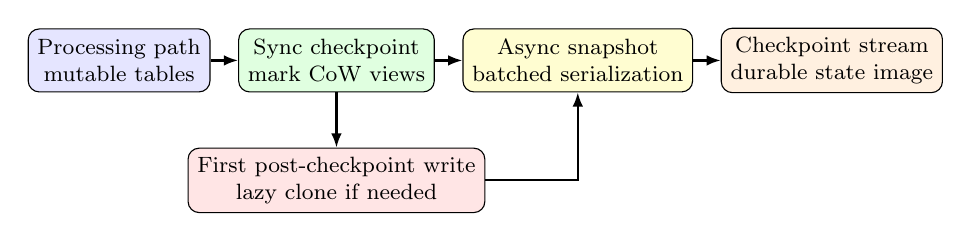
\begin{tikzpicture}[
    font=\footnotesize,
    phasebox/.style={draw, rounded corners, align=center, minimum width=2.15cm, minimum height=0.8cm},
    arrow/.style={-{Latex[length=1.8mm]}, thick}
  ]
  \node[phasebox, fill=blue!10] (run) {Processing path\\mutable tables};
  \node[phasebox, fill=green!12, right=0.35cm of run] (cow) {Sync checkpoint\\mark CoW views};
  \node[phasebox, fill=yellow!18, right=0.35cm of cow] (async) {Async snapshot\\batched serialization};
  \node[phasebox, fill=orange!12, right=0.35cm of async] (store) {Checkpoint stream\\durable state image};
  \node[phasebox, fill=red!10, below=0.7cm of cow, minimum width=2.4cm] (mut) {First post-checkpoint write\\lazy clone if needed};

  \draw[arrow] (run) -- (cow);
  \draw[arrow] (cow) -- (async);
  \draw[arrow] (async) -- (store);
  \draw[arrow] (cow) -- (mut);
  \draw[arrow] (mut.east) -| ($(async.south)+(0,-0.3)$) -| (async.south);
\end{tikzpicture}%
}
\caption{Checkpoint path in \system. Synchronous capture creates immutable CoW views with minimal blocking, while asynchronous serialization drains those views in batches. The first post-checkpoint mutation may trigger a lazy clone.}
\label{fig:snapshot}
\end{figure}

This checkpoint structure also affects engineering trade-offs. CoW snapshots preserve a compact online layout, but they also mean that post-checkpoint write bursts can briefly increase memory pressure if many tables are mutated immediately after capture. The implementation therefore benefits most when checkpoint intervals are moderate and write bursts are not perfectly synchronized across all key-groups.

\subsection{Restore Path and Compatibility}

The restore path reconstructs state by iterating over checkpointed key-groups and rehydrating the corresponding tables. The implementation uses Flink-compatible metadata and serialization proxies so that state descriptors, key serializers, and namespace/value serializers are restored consistently with Flink's standard keyed-state machinery. The practical result is compatibility at the API level and consistent behavior under checkpoint/savepoint round-trips.

Correctness evidence from the delivery report is consistent with this design. Across 184 tests, including 54 JVM-side tests and 130 native-engine tests, the system covers the major keyed-state abstractions, snapshot consistency, namespace behavior, rescaling, serialization round-trips, and native data-structure correctness.

\section{Implementation Details}

\subsection{Backend Construction and Key Context}

The backend is organized around a keyed backend builder and a compact key context. The current key and current key-group index are made directly accessible to the state implementations so that repeated accesses can avoid unnecessary wrapper calls. This matters because the dominant operations in ValueState-heavy workloads are extremely short; if the surrounding framework adds even small layers of indirection, the storage optimizations become harder to observe in end-to-end behavior.

\subsection{Native Execution Path}

In addition to the Java-path implementation, the repository includes a native state engine that stores state in off-heap Swiss tables and exposes operations through JNI. This path allows the system to explore lower-level memory control and architecture-specific implementations while preserving the same logical state abstractions. The native codebase includes its own test suite, storage specialization, and bug-fix history, including correctness fixes for control-byte cloning and empty-slot detection.

The paper does not claim that the native path alone explains all observed speedups. Instead, it serves as an implementation vehicle for off-heap state management and compact data-structure control. On Intel, the strongest gains arise even without platform-specific hardware support, suggesting that layout and access-path design are the dominant factors in the reported workload improvements.

The native path is also operationally more nuanced than a plain JNI wrapper. The repository supports a dual-mode execution model: a platform-specific mode when the target memory facility is available, and a simulation mode for development and validation. Allocation APIs cover regular and aligned blocks, and the more recent raw-pool strategy avoids allocating many isolated large mappings by routing requests through a shared allocation path. This detail matters because keyed state is naturally fragmented across many key-groups and namespaces; if the allocator treats each unit as an isolated large reservation, scalability suffers before the state logic itself becomes a bottleneck.

At the C++ layer, the repository includes a fuller native state engine whose Swiss-table implementation uses wider group-based matching and exposes state operations through a thin JNI bridge. Even when that path is not the default in every reported benchmark, it is part of the paper's evidence that the design generalizes beyond one Java data structure. The associated bug-fix history is also instructive: correctness issues around control-byte cloning, sentinel handling, and CoW-before-erase behavior had to be resolved before the backend could be trusted under checkpointed mutations. In other words, the systems problem is not only to make the data path fast, but also to preserve exact state semantics under cloning, deletion, and restore.

\subsection{Operational Characteristics}

Several implementation characteristics recur across the repository and evaluation artifacts.
\begin{itemize}
\item \textbf{Minimal routing on the hot path}: void namespaces skip one map lookup per state access.
\item \textbf{Compact metadata}: control bytes and payload arrays reduce pointer chasing.
\item \textbf{Specialization where it matters}: primitive-key tables remove boxing on common paths.
\item \textbf{Checkpoint-aware storage}: CoW capture and batched serialization keep the snapshot protocol compatible without flattening the in-memory layout.
\end{itemize}

These choices are small individually, but the evaluation indicates that their combination is large enough to change both throughput and runtime stability.

\subsection{Compatibility and Deployment Constraints}

The repository's delivery and usage documents make two deployment constraints explicit. First, the backend is expected to be discovered by Flink through SPI and to remain compatible with Flink 1.20.3 state-backend interfaces and checkpoint/savepoint protocols. Second, when the native engine is enabled, the TaskManager process must load the accompanying native library explicitly, which means operational packaging matters for production deployment even if user jobs remain unchanged.

These constraints shape the implementation in practical ways. Serializer and metadata proxies cannot be treated as internal details because they must survive checkpoint round-trips. Likewise, the native path cannot assume a monolithic deployment environment; it must coexist with regular Flink process startup, class loading, and containerized execution. In other words, a fast backend is only useful if it can be built, shipped, loaded, and restored within normal Flink operations.

\begin{table}[t]
\caption{Operational constraints that influence \system deployment.}
\label{tab:ops}
\centering
\small
\begin{tabularx}{\columnwidth}{L{2.15cm}Y}
\toprule
Constraint & Implication \\
\midrule
SPI discovery & The backend must be packaged so Flink can load it without user-job changes \\
Native library loading & TaskManager startup must expose the native library path when the off-heap engine is enabled \\
Process memory sizing & TaskManager process memory and managed memory must be balanced so native/off-heap state has room to grow \\
Checkpoint compatibility & Serializer metadata and state descriptors must survive checkpoint/savepoint round-trips unchanged \\
Container deployment & JobManager and TaskManager images must carry both the backend JAR and the native runtime artifacts \\
\bottomrule
\end{tabularx}
\end{table}

\section{Experimental Methodology}

\subsection{Platforms and Baselines}

The evaluation uses two hardware environments captured in the repository artifacts. The first is an Intel x86\_64 reference platform used for operator-level and workload-level comparisons. The second is a Kunpeng aarch64 platform used to study behavior under a different microarchitectural profile. The comparison baseline throughout is Flink's heap-based keyed state backend, with RocksDB serving as a relevant design point in the discussion but not as the direct baseline in the reported benchmark figures.

The software stack targets Flink 1.20-series keyed state interfaces and standard checkpointing. All experiments use the same application-level logic across backends so that differences can be attributed to the state path rather than to operator rewrites.

\begin{table*}[t]
\caption{Experimental setup summary from repository documentation and delivery artifacts.}
\label{tab:setup}
\centering
\small
\begin{tabularx}{\textwidth}{L{2.1cm}L{3.1cm}Y}
\toprule
Category & Setting & Notes \\
\midrule
Software stack & Apache Flink 1.20.3, Java 8+, containerized standalone deployment & Same application logic across backends; checkpoint/savepoint semantics preserved \\
Default cluster & 1 JobManager (2 cores, 8~GB) + 2 TaskManagers (4 cores, 16~GB each), total parallelism 8 & Reported as the default benchmark topology in the delivery document \\
Kunpeng platform & aarch64, openEuler, TaskManager heap 11.7~GB, managed memory 512~MB, 4-core TM limit for NexMark & Used to study the off-heap/native path under a different microarchitectural profile \\
Intel platform & x86\_64 reference platform, TaskManager memory sweep of 16/18/20~GB with 12/14/15~GB heap for NexMark & Used for WordCount, operator-level benchmarks, NexMark scans, and VTune analysis \\
WordCount sweep & 36 points over key cardinality and skew, each run processes $2\times10^9$ records & Isolates repeated ValueState read-modify-write behavior \\
State benchmark & Retained ValueState, ListState, and MapState operations on Intel & Isolates point updates, lookups, iteration, and removal \\
NexMark & Queries q4, q5, q8, q9, q11, q18, q19, q20 under multiple memory budgets & Highlights state-heavy query behavior and runtime stability \\
\bottomrule
\end{tabularx}
\end{table*}

The resulting setup is deliberately pragmatic. It combines controlled microbenchmarks with end-to-end query workloads and uses the same backend implementation in both cases. This matters because some backend effects are only visible in tight loops, while others emerge only when checkpointing, GC, and operator scheduling interact in a full pipeline.

\subsection{Workloads}

We use three workload families.
\begin{itemize}
\item \textbf{WordCount grid sweep}: a ValueState-dominated microbenchmark that scans combinations of key cardinality and skew to isolate the repeated read-modify-write path.
\item \textbf{Flink operator-level state benchmark}: a JMH-style benchmark over representative ValueState, ListState, and MapState operations.
\item \textbf{NexMark}: end-to-end streaming queries with windows, ranking, joins, and other state-intensive patterns.
\end{itemize}

The workload set is intentionally layered: the state benchmark isolates operator cost, WordCount isolates repeated keyed-state access under controlled distributions, and NexMark shows how those effects persist once embedded in realistic streaming pipelines.

The benchmark harnesses also matter. The WordCount benchmark in the repository disables checkpointing by default so that the measured throughput reflects steady-state state access rather than periodic CoW overhead. Checkpointing can be re-enabled parametrically, but the default benchmark mode isolates the access path itself. This is appropriate for the paper because checkpoint behavior is studied separately through the design analysis, correctness artifacts, and end-to-end workloads where checkpoint interaction is part of normal execution.

\subsection{Metrics}

The evaluation reports throughput, query execution time, selected stability outcomes under tight memory budgets, and microarchitectural indicators collected through Intel VTune and Linux profiling. For checkpoint behavior and correctness, the evaluation relies on the repository's delivery report and test artifacts.

One limitation of the evaluation is that the two platforms are not used as strict apples-to-apples hardware comparisons; they are used to expose how the same backend behaves under different processor and runtime conditions. This is acceptable for the present paper because the claim is about backend behavior under realistic deployment targets, not about one processor family being intrinsically superior.

\section{Experimental Results}

\subsection{Correctness and Compatibility}

Table~\ref{tab:tests} summarizes the top-level correctness evidence. The repository's delivery report records 54 JVM tests and 130 native-engine tests, all passing. The covered behaviors include ValueState, ListState, MapState, ReducingState, AggregatingState, checkpoint/savepoint round-trips, namespace behavior, rescaling, SPI loading, and native data-structure correctness.

\begin{table}[t]
\caption{Top-level correctness evidence from repository test artifacts.}
\label{tab:tests}
\centering
\small
\begin{tabularx}{\columnwidth}{L{2.2cm}C{1.5cm}Y}
\toprule
Suite & Count & Scope \\
\midrule
JVM tests & 54 & State API semantics, checkpoint/savepoint behavior, windowed workloads, SPI loading \\
Native tests & 130 & Swiss-table correctness, snapshot consistency, serialization, native lifecycle and stress \\
Total & 184 & Combined correctness and compatibility evidence \\
\bottomrule
\end{tabularx}
\end{table}

The result is important for the rest of the evaluation. A state backend that optimizes the hot path but diverges from Flink semantics would not be usable in practice. The test suite suggests that \system preserves the required interface behavior while still changing the physical state layout aggressively.

Table~\ref{tab:semantics} adds representative semantic coverage examples. These cases matter because many backend optimizations fail not on the common path, but on API corner cases such as null handling, namespace isolation, or interaction between clear and internal caches.

\begin{table*}[t]
\caption{Representative semantic and compatibility checks covered by repository tests.}
\label{tab:semantics}
\centering
\small
\begin{tabularx}{\textwidth}{L{2.1cm}L{2.6cm}Y}
\toprule
Category & Representative checks & Purpose \\
\midrule
ValueState semantics & default read returns null, update(null) clears, multiple ValueState instances remain independent & Preserves Flink's point-state contract and state isolation \\
ListState boundaries & add(null) and update(null) reject invalid inputs, update(empty) clears state, append path avoids unnecessary list recreation & Checks API corner cases and validates optimized append behavior \\
MapState semantics & generic and typed inner-map paths, null values remain visible, entry count tracks inserts and deletes & Confirms compatibility of fine-grained map operations and accounting \\
Namespace behavior & TimeWindow namespace tests, multiple namespaces under COW snapshot, windowed aggregation restore & Verifies that namespace-aware routing remains correct under snapshot and restore \\
Operational integration & SPI auto-discovery, skewed high-load ValueState, sliding event-time window WordCount & Confirms backend usability under realistic operator entry points \\
Snapshot correctness & snapshot sees old values, snapshot includes deletes, release and re-snapshot, checkpoint round-trip consistency & Validates CoW semantics under overwrite, delete, and restore \\
\bottomrule
\end{tabularx}
\end{table*}

\subsection{WordCount Grid Sweep}

The WordCount benchmark isolates the repeated ValueState sequence of reading a counter, incrementing it, and writing it back. This makes it a good workload for revealing how a backend behaves once the state path dominates operator cost.

Figure~\ref{fig:wc-speedup} shows the Intel grid sweep as a speedup map over key cardinality and skew. The delivery report states that \system outperforms the heap backend on all 36 scanned points, with a minimum speedup of 1.024$\times$, a maximum of 1.414$\times$, and an average of 1.270$\times$. For runs of $2\times 10^9$ records, this corresponds to an average end-to-end reduction of about 37 seconds per configuration.

\begin{figure*}[t]
\centering
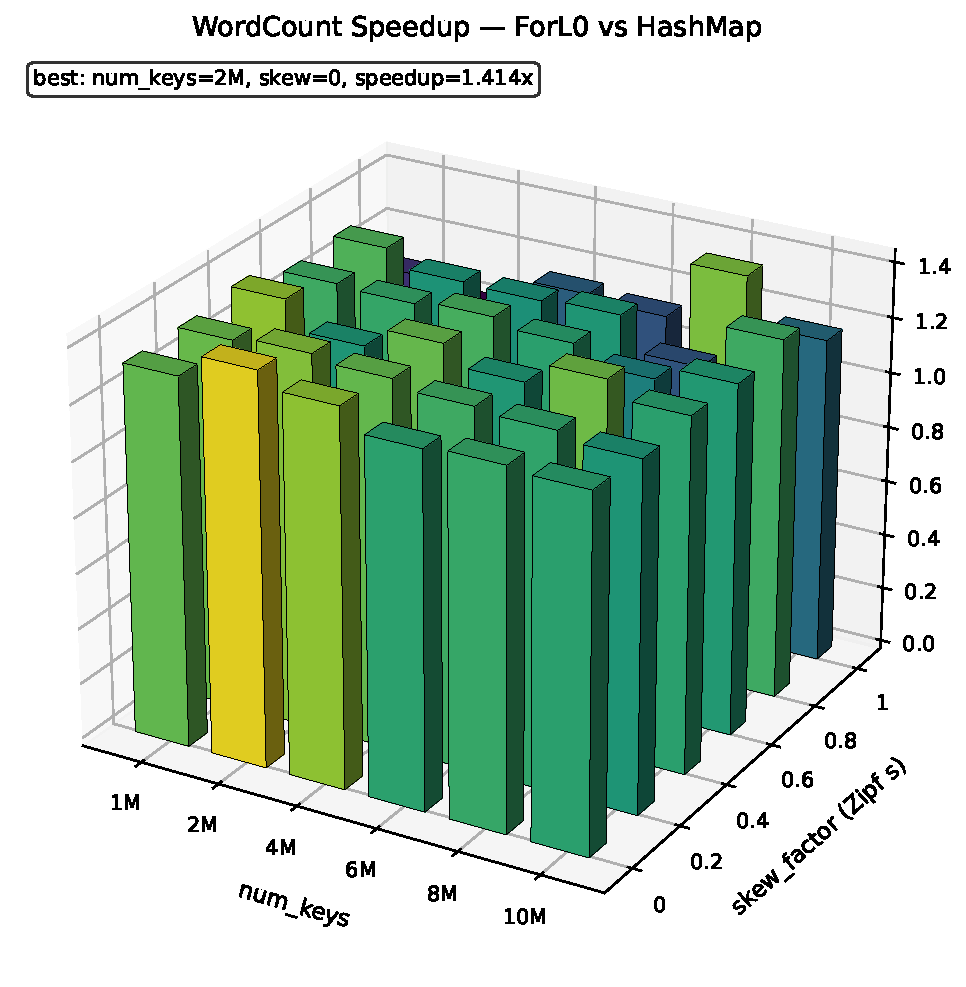
\includegraphics[width=0.72\textwidth]{wordcount_grid_speedup.pdf}
\caption{Intel WordCount grid-sweep speedup of \system over the heap backend across key-cardinality and skew configurations. All 36 scanned points favor \system, with a 1.270$\times$ average and 1.414$\times$ peak speedup.}
\label{fig:wc-speedup}
\end{figure*}

To make the trend more concrete, Table~\ref{tab:wordcount-points} lists representative scan points from the 36-point grid. The table shows that the improvement is not confined to one narrow configuration. Moderate skew, weak skew, and fully hot-keyed cases all benefit, although the improvement is largest away from the most extreme hot-key setting.

\begin{table*}[t]
\caption{Representative Intel WordCount grid-sweep points from the 36-point scan. Throughput is reported in M records/s.}
\label{tab:wordcount-points}
\centering
\small
\begin{tabular}{C{1.4cm}C{1.0cm}C{1.5cm}C{1.5cm}C{1.3cm}C{1.4cm}}
\toprule
Keys & Skew & Heap & \system & Speedup & Time reduction \\
\midrule
1M & 0.0 & 13.153 & 17.464 & 1.328$\times$ & 37.54~s \\
2M & 0.0 & 12.140 & 17.170 & 1.414$\times$ & 48.26~s \\
4M & 0.4 & 9.657 & 12.858 & 1.332$\times$ & 51.57~s \\
6M & 0.8 & 10.556 & 13.297 & 1.260$\times$ & 39.05~s \\
8M & 1.0 & 11.162 & 15.028 & 1.346$\times$ & 46.10~s \\
10M & 0.2 & 9.933 & 12.476 & 1.256$\times$ & 41.04~s \\
10M & 1.0 & 12.616 & 14.855 & 1.178$\times$ & 23.90~s \\
\bottomrule
\end{tabular}
\end{table*}

Figure~\ref{fig:wc-absolute} shows the same WordCount sweep as absolute throughput surfaces for the heap baseline and \system. The figure makes one additional point that the speedup heatmap alone does not: \system does not win merely because the baseline collapses at a few outliers. The absolute throughput surface is elevated across most of the scanned space.

\begin{figure*}[t]
\centering
\begin{minipage}[t]{0.48\textwidth}
\centering
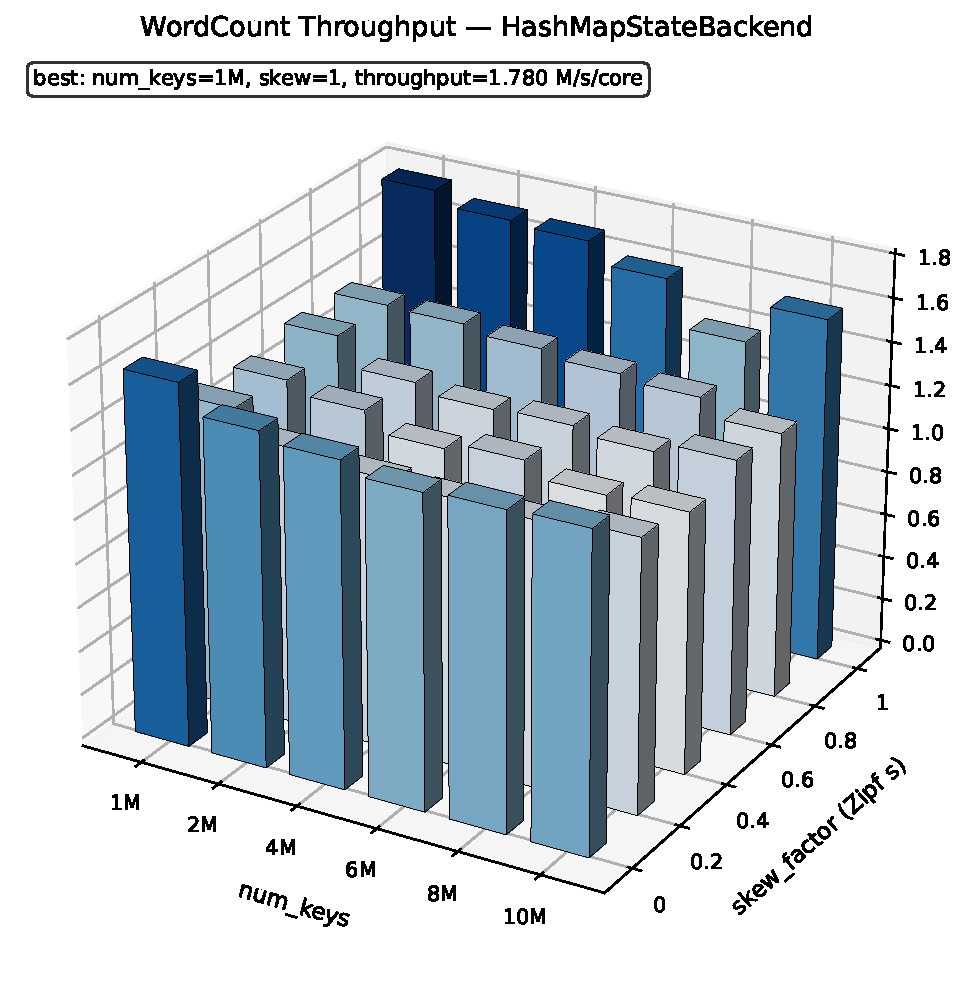
\includegraphics[width=\linewidth]{wordcount_grid_hashmap.pdf}
\end{minipage}\hfill
\begin{minipage}[t]{0.48\textwidth}
\centering
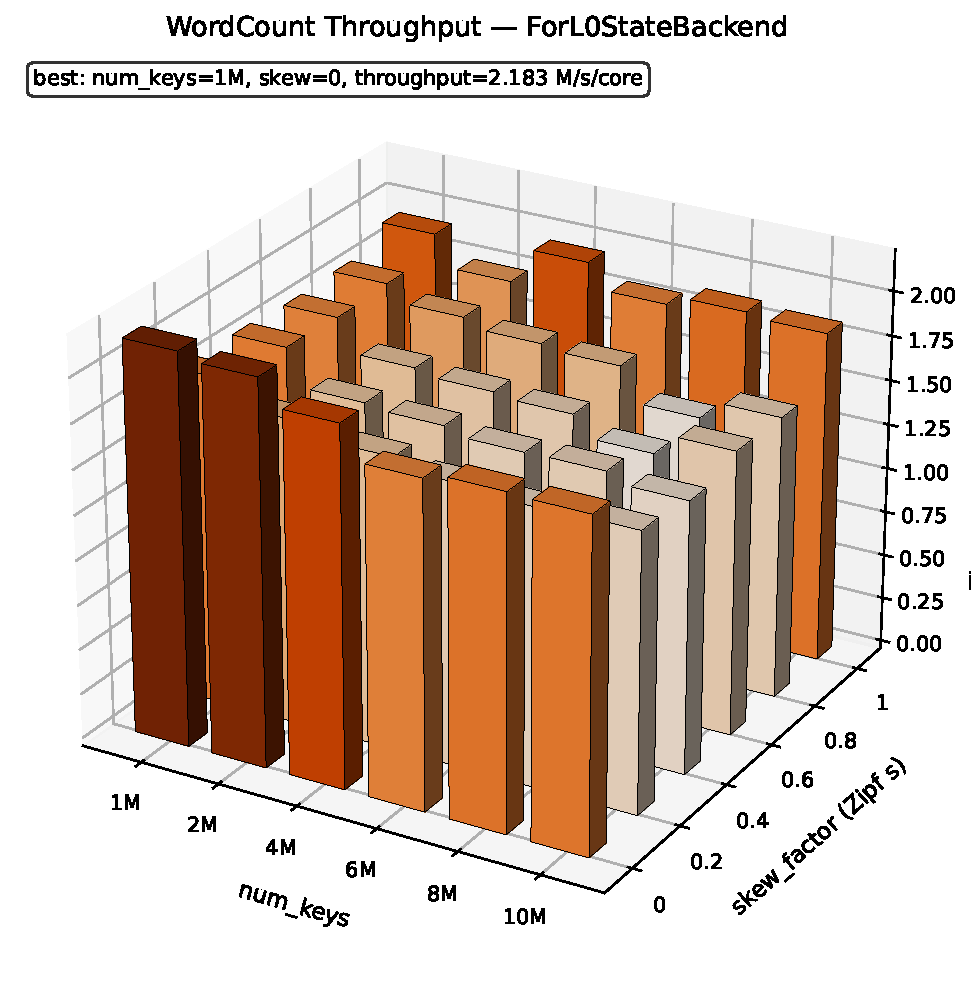
\includegraphics[width=\linewidth]{wordcount_grid_forl0.pdf}
\end{minipage}
\caption{Absolute Intel WordCount throughput surfaces. Left: heap baseline. Right: \system. The gain is broadly distributed across the scanned key-cardinality/skew grid rather than concentrated in a small number of pathological points.}
\label{fig:wc-absolute}
\end{figure*}

For reproducibility, Table~\ref{tab:wordcount-detail} provides a denser slice of the Intel scan. The table complements the heatmaps by exposing raw throughput and time deltas across a wider set of representative points.

\begin{table*}[t]
\caption{Expanded Intel WordCount sample from the grid sweep. Throughput is reported in M records/s.}
\label{tab:wordcount-detail}
\centering
\scriptsize
\begin{tabular}{C{1.2cm}C{0.9cm}C{1.4cm}C{1.4cm}C{1.2cm}C{1.4cm}}
\toprule
Keys & Skew & Heap & \system & Speedup & Time reduction \\
\midrule
1M & 0.0 & 13.153 & 17.464 & 1.328$\times$ & 37.54~s \\
1M & 0.4 & 10.786 & 14.673 & 1.360$\times$ & 49.12~s \\
1M & 0.8 & 11.128 & 14.627 & 1.314$\times$ & 43.00~s \\
1M & 1.0 & 14.243 & 15.471 & 1.086$\times$ & 11.15~s \\
2M & 0.0 & 12.140 & 17.170 & 1.414$\times$ & 48.26~s \\
2M & 0.4 & 10.364 & 13.033 & 1.258$\times$ & 39.52~s \\
2M & 0.8 & 11.080 & 13.887 & 1.253$\times$ & 36.49~s \\
2M & 1.0 & 13.740 & 14.068 & 1.024$\times$ & 3.40~s \\
4M & 0.0 & 11.812 & 16.040 & 1.358$\times$ & 44.63~s \\
4M & 0.4 & 9.657 & 12.858 & 1.332$\times$ & 51.57~s \\
4M & 0.8 & 10.813 & 13.487 & 1.247$\times$ & 36.66~s \\
4M & 1.0 & 13.595 & 15.704 & 1.155$\times$ & 19.76~s \\
8M & 0.0 & 11.494 & 14.853 & 1.292$\times$ & 39.34~s \\
8M & 0.4 & 9.388 & 12.560 & 1.338$\times$ & 53.80~s \\
8M & 0.8 & 10.364 & 11.791 & 1.138$\times$ & 23.35~s \\
8M & 1.0 & 11.162 & 15.028 & 1.346$\times$ & 46.10~s \\
\bottomrule
\end{tabular}
\end{table*}

The same delivery report records a contrasting result on Kunpeng: the average WordCount speedup is approximately 0.96, indicating rough parity rather than a systematic gain. This asymmetry is useful rather than inconvenient. It shows that the design is not simply ``faster everywhere''; the main benefits appear when the target platform rewards compact metadata and regular probing, while other platforms may expose JNI or architecture-specific costs that offset those gains.

Another useful pattern is that \system does not collapse under strong skew. The hot-key endpoint at skew 1.0 still favors \system across every tested key cardinality. This suggests that the backend's compact routing and control-byte probing remain beneficial even when the workload becomes increasingly repetitive and logically simple.

\subsection{Operator-Level State Benchmark}

Figure~\ref{fig:microbench-tkde} reports operator-level results from the Flink state benchmark on Intel. Of the 14 original operator points, 13 retained operations favor \system. The strongest gains are +132\% for ListState iteration, +110\% for MapState insertion, +91\% for MapState lookup, +87\% for ValueState insertion, and +74\% for MapState removal.

\begin{figure*}[t]
\centering
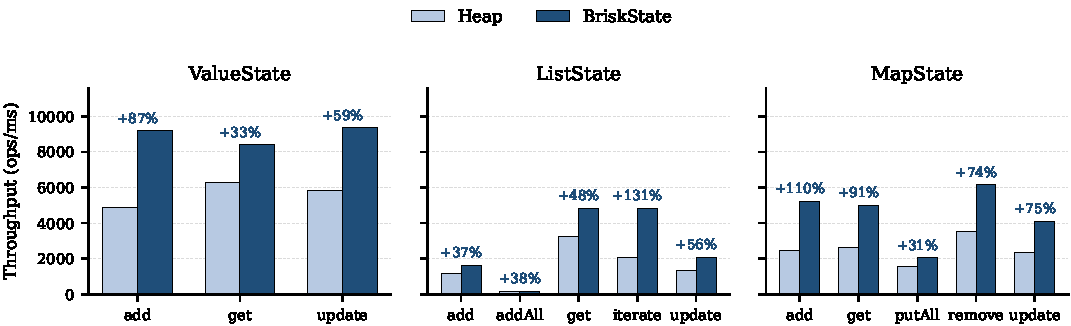
\includegraphics[width=0.82\textwidth]{flink_state_benchmark_intel.pdf}
\caption{Operator-level Intel Flink state benchmark. \system improves the dominant update, lookup, iteration, and removal paths across retained ValueState, ListState, and MapState operations.}
\label{fig:microbench-tkde}
\end{figure*}

These gains support the core design hypothesis. The benchmark does not include end-to-end pipeline effects, so its improvements are best interpreted as evidence that the state-access path itself has become cheaper before any pipeline-level interactions are considered.

\begin{table}[t]
\caption{Representative operator-level gains from the Intel state benchmark.}
\label{tab:jmh-summary}
\centering
\small
\begin{tabular}{L{2.2cm}C{1.2cm}}
\toprule
Operation & Gain \\
\midrule
ListState get+iterate & +131.5\% \\
MapState add & +110.0\% \\
MapState get & +91.0\% \\
ValueState add & +87.2\% \\
MapState remove & +74.0\% \\
\bottomrule
\end{tabular}
\end{table}

The distribution of these gains is consistent with the implementation details discussed earlier. ValueState benefits from the short routing path and compact point lookup. MapState benefits when the backend can operate on typed inner entries rather than materializing a full serialized map blob. ListState iteration benefits when compact payload layout reduces overhead during sequential traversal.

\subsection{End-to-End NexMark Results}

Figure~\ref{fig:nexmark-tkde} reports end-to-end results on representative NexMark queries. The figure contains two distinct messages.

First, tight-memory configurations reveal the backend most clearly. On Intel with 16~GB task-manager memory, the delivery report records that state-intensive queries such as q4 and q9 fall from 352~s and 232~s on the heap backend to 61~s and 46~s under \system. The same report notes that q19 and q20, which become stuck under the heap baseline in the same configuration, complete successfully under \system.

Second, as heap budgets become more generous, the difference narrows for some queries. This is expected: once GC pressure is relaxed, the heap backend recovers some performance. Nevertheless, \system remains more stable across the tested configurations and avoids the extreme tail behaviors observed under constrained budgets.

Table~\ref{tab:nexmark} complements Figure~\ref{fig:nexmark-tkde} with the exact runtime values reported in the delivery document. The table is useful because the figure highlights trends, while the table reveals where the backend changes query feasibility as well as query speed.

\begin{table*}[t]
\caption{Selected NexMark runtimes from the repository delivery report. ``Stuck'' indicates that the heap backend failed to complete in the tested Intel 16~GB configuration.}
\label{tab:nexmark}
\centering
\scriptsize
\begin{tabularx}{\textwidth}{L{2.4cm}C{0.8cm}C{0.8cm}C{0.8cm}C{0.8cm}C{0.8cm}C{0.8cm}C{0.8cm}C{0.8cm}}
\toprule
Configuration & q4 & q5 & q8 & q9 & q11 & q18 & q19 & q20 \\
\midrule
Kunpeng heap (11.7~GB heap) & 716~s & 103~s & 72~s & 201~s & 98~s & 134~s & 638~s & 542~s \\
Kunpeng \system & 147~s & 103~s & 62~s & 105~s & 96~s & 93~s & 119~s & 91~s \\
Intel heap (16~GB TM / 12~GB heap) & 352~s & 63~s & 39~s & 232~s & 44~s & 53~s & stuck & stuck \\
Intel \system\ (16~GB TM / 12~GB heap) & 61~s & 56~s & 36~s & 46~s & 35~s & 34~s & 47~s & 40~s \\
Intel heap (18~GB TM / 14~GB heap) & 156~s & 64~s & 36~s & 46~s & 53~s & 53~s & 279~s & 313~s \\
Intel \system\ (18~GB TM / 14~GB heap) & 57~s & 52~s & 36~s & 46~s & 37~s & 38~s & 45~s & 38~s \\
Intel heap (20~GB TM / 15~GB heap) & 57~s & 64~s & 38~s & 45~s & 37~s & 61~s & 123~s & 84~s \\
Intel \system\ (20~GB TM / 15~GB heap) & 57~s & 52~s & 36~s & 45~s & 37~s & 35~s & 43~s & 38~s \\
\bottomrule
\end{tabularx}
\end{table*}

\begin{figure*}[t]
\centering
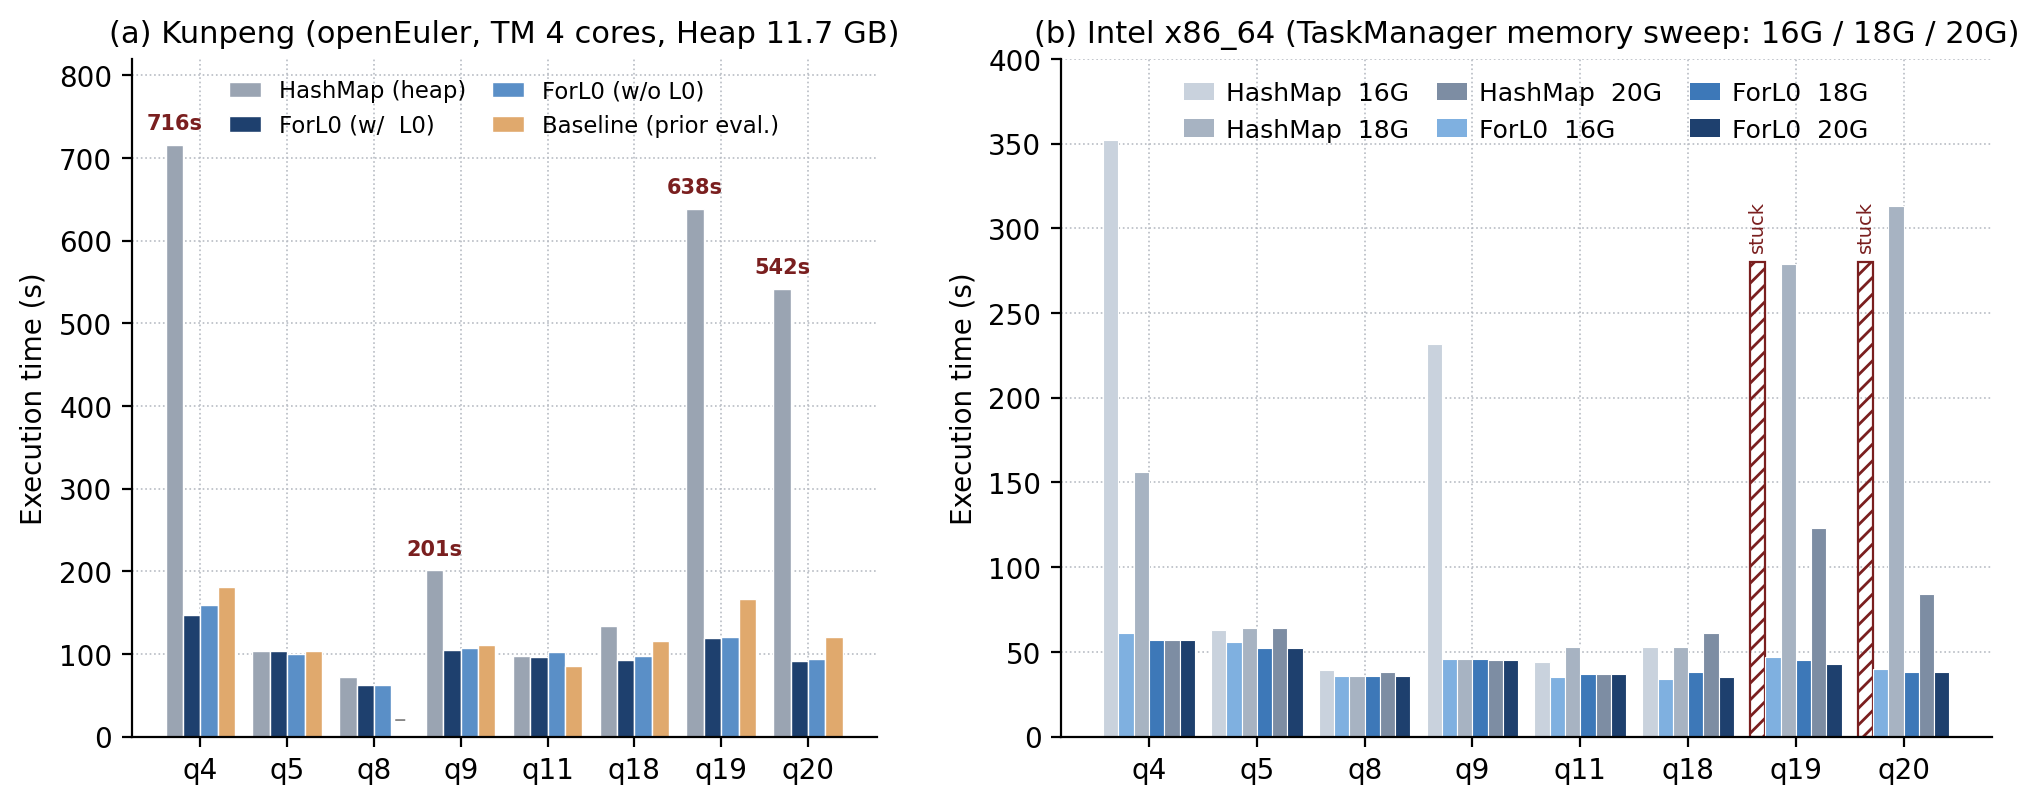
\includegraphics[width=0.96\textwidth]{nexmark_comparison.png}
\caption{End-to-end NexMark behavior across Kunpeng and Intel platforms. \system provides the largest gains under memory-constrained, state-intensive configurations and avoids several stuck or severely GC-affected cases observed with the heap backend.}
\label{fig:nexmark-tkde}
\end{figure*}

The Kunpeng results are also informative. Under the reported heap budget of 11.7~GB, q4, q9, q19, and q20 drop from severe heap-backend slowdowns to 147~s, 105~s, 119~s, and 91~s respectively under \system. At the same time, the report concludes that the dominant benefit on Kunpeng is system-level heap-pressure relief rather than the full algorithmic speedup seen on Intel microbenchmarks.

The Intel memory sweep reinforces that interpretation. As the TaskManager budget grows from 16~GB to 20~GB, the heap baseline recovers sharply on q4 and the stuck cases disappear, while \system remains comparatively flat. That pattern is hard to explain by algorithmic complexity alone; it is more consistent with a backend that avoids heap blow-up and therefore avoids the regime in which GC dominates useful work.

There is also a state-type interpretation hidden in these results. The delivery report notes that the extra platform-specific cache layer contributes only modestly to NexMark on Kunpeng, which suggests that the main end-to-end gain in these queries comes from moving large state structures off the managed heap and stabilizing ListState and MapState behavior under memory pressure. This contrasts with WordCount, where the dominant state abstraction is ValueState and the benefit is easier to attribute to direct point-access efficiency.

\subsection{Microarchitectural Analysis}

Table~\ref{tab:vtune} summarizes the VTune WordCount analysis reported for the Intel platform. The figures show that the performance gain is not merely a wall-clock artifact. Memory Bound falls from 48.1\% to 15.3\%, DRAM Bound from 30.8\% to 2.2\%, and CPI from 0.615 to 0.375, while Instructions Retired increase from $1.98\times 10^{12}$ to $3.49\times 10^{12}$ in the same 60.001-second window.

\begin{table}[t]
\caption{Selected VTune WordCount metrics before and after the optimized \system path on Intel.}
\label{tab:vtune}
\centering
\small
\begin{tabular}{L{2.15cm}C{1.1cm}C{1.1cm}C{1.0cm}}
\toprule
Metric & Before & After & Change \\
\midrule
Instructions Retired & $1.98\times 10^{12}$ & $3.49\times 10^{12}$ & 1.76$\times$ \\
CPI Rate & 0.615 & 0.375 & $\downarrow$39\% \\
Retiring & 30.4\% & 50.9\% & +20.5pp \\
Memory Bound & 48.1\% & 15.3\% & $\downarrow$32.8pp \\
DRAM Bound & 30.8\% & 2.2\% & $\downarrow$28.6pp \\
Back-End Bound & 58.1\% & 29.5\% & $\downarrow$28.6pp \\
\bottomrule
\end{tabular}
\end{table}

Taken together with the operator-level benchmark, the VTune analysis supports a consistent interpretation: \system primarily improves data access locality and reduces long-latency memory traffic on the hot path.

\subsection{Cross-Platform Synthesis}

The combined results suggest a two-level interpretation. On Intel, \system improves both the algorithmic efficiency of the in-memory access path and the runtime stability of memory-intensive jobs. On Kunpeng, the strongest visible effect is stability under constrained heap budgets, while pure WordCount speedups are much smaller. This distinction matters because it shows that the same backend can be valuable for different reasons on different platforms.

More concretely, the backend appears to help on Intel by shortening probe paths and reducing high-latency memory traffic, while on Kunpeng it helps chiefly by preventing heap-resident state from dominating GC behavior in state-heavy jobs. The design is therefore best understood as a backend that improves physical state organization; the exact manifestation of that improvement depends on the platform and workload.

\section{Discussion}

The evaluation suggests that the largest benefits of \system arise under two conditions: when keyed state is accessed repeatedly enough that layout overhead becomes visible on every record, and when memory budgets are tight enough that heap-resident state becomes unstable. This explains why the operator-level benchmark and Intel WordCount sweep show clean improvements, while the Kunpeng WordCount sweep is much flatter and NexMark gains become largest in the configurations where the heap baseline experiences GC pressure or execution instability.

These findings also clarify the role of the backend relative to the application. A state backend does not change the logical query plan, but it changes the physical cost of every state access and every snapshot boundary. Once workload structure and memory budget make those costs visible, backend design becomes a first-order systems concern.

The evaluation also highlights a useful lesson for benchmark methodology. No single benchmark is sufficient to characterize a state backend. Operator-level tests reveal whether point operations became cheaper, WordCount reveals whether those savings survive repeated per-record state updates, and NexMark reveals whether the same backend still behaves well when windows, joins, checkpointing, and memory pressure interact. The combination is what allows the paper to attribute the observed gains to state layout rather than to one narrow workload artifact.

There is an additional design lesson here for backend builders. Many state backends are discussed as if they were primarily persistence mechanisms, with runtime overhead treated as a secondary matter. The results in this paper suggest a different emphasis: once stateful streaming jobs spend most of their time traversing in-memory state, the backend becomes part of the execution engine itself. Probe structure, routing depth, serializer boundaries, and snapshot interference are then no longer storage details; they are execution-path decisions. This is why relatively small structural changes such as void-namespace bypass, packed control metadata, or typed inner-map access can surface as meaningful end-to-end differences under the right workload conditions.

The same point helps explain why a backend can look unremarkable under one workload and decisive under another. If a job performs only occasional keyed updates and spends most of its time elsewhere, even a well-designed state backend will not dominate runtime. But when the job repeatedly alternates between user logic and short state touches, or when the heap baseline drifts into a GC-dominated regime, backend design becomes much more visible. This conditional visibility is not a weakness in the evidence; it is part of the phenomenon being studied. Journal-style evaluation is especially important here because it can layer multiple workloads and isolate exactly when the backend becomes first-order.

The current implementation still leaves room for future improvement. The platform asymmetry indicates that architecture-specific paths and JNI overhead require further tuning on Kunpeng-class processors. Likewise, the operator-level outlier in the Flink state benchmark suggests that not every state pattern benefits equally from the current layout choices. These are useful constraints for subsequent work rather than contradictions of the main results.

Another limitation is that the current evaluation emphasizes read/update-heavy keyed state and selected NexMark queries rather than broader mixes of timers, large-window eviction patterns, and heavily write-amplified checkpoint schedules. Those cases remain important future work, particularly if the backend is extended toward wider production deployment.

\subsection{Checkpoint Format and Migration Implications}

The implementation also exposes a practical boundary that matters in real deployments: compact in-memory layout and checkpoint interoperability are related but not identical concerns. The backend supports regular checkpoint and savepoint flows through Flink-compatible metadata handling, but the codebase explicitly distinguishes its custom full-checkpoint path from Flink's canonical savepoint format during restore. This is a sensible engineering compromise. It allows the online state layout and serialization path to remain efficient while still preserving migration through supported restore mechanisms rather than forcing the online representation to mimic one canonical byte layout.

That distinction has operational implications. For routine fault tolerance inside one deployment family, the backend can optimize around its own full snapshot format and asynchronous writer. For migration between backends or across deployment topologies, canonical savepoints remain the safer interchange point because they decouple execution-time layout from the persisted interchange format. This is not a weakness of \system in particular; it is a recurring tension in stateful systems that try to optimize the in-memory path without giving up portability.

From a systems perspective, this means that backend evaluation should not stop at throughput. The real question is whether a backend can maintain a compact fast path while still participating cleanly in the lifecycle that matters to operators: startup, checkpoint, restore, rescale, and controlled migration. The evidence in the repository suggests that \system is already strong on the first four and has clear operational guidance for the last one.

\subsection{Broader Applicability}

Although the evaluation focuses on WordCount and NexMark, the design is relevant to a wider class of Flink workloads. Many SQL and Table API pipelines ultimately devolve to repeated access over keyed aggregates, window state, and small per-key collections. In those settings, the same ingredients that matter here remain relevant: whether void namespaces bypass extra routing, whether compact control metadata filters candidates before payload access, and whether snapshot capture interrupts the hot path minimally.

The codebase hints at this broader applicability through components such as binary row conversion utilities, typed inner-map support, and windowed namespace tests. These implementation surfaces are easy to overlook when reading benchmark summaries, but they are exactly what determines whether a backend can move from a microbenchmark success to a usable substrate for higher-level relational and event-time operators. In other words, the paper's results should be read as evidence for a backend design pattern, not only for one benchmark-specific optimization.

This perspective also suggests several next steps for future work. One is to extend the evaluation toward timer-heavy pipelines and incremental or differential checkpoint styles. Another is to study whether platform-specific SIMD paths and JNI batching can narrow the remaining gap between the backend's Intel and Kunpeng behavior. A third is to examine how far typed fast paths can be pushed for composite SQL-style keys and values before serializer fallback becomes dominant again. Each direction follows directly from the current results and would strengthen the case that layout-aware state backends deserve a more central place in stream-processing systems research.

\section{Threats to Validity}

The evaluation is grounded in repository benchmarks and delivery artifacts rather than in a freshly instrumented cross-laboratory campaign, so it inherits the strengths and limits of those artifacts. The strongest threat is platform asymmetry: Intel and Kunpeng are used to expose behavior under different architectural conditions, but they are not controlled to the point where every runtime factor is identical. The paper therefore avoids claims about one processor family being universally better and instead focuses on how the backend behaves under the tested targets.

The second threat is workload coverage. WordCount and the Flink state benchmark strongly illuminate repeated keyed-state access, while NexMark exercises broader streaming logic, but there remain other important patterns such as timer-heavy workloads, very large namespace churn, and checkpoint-heavy deployment schedules. The paper should therefore be read as evidence that state layout matters materially for representative keyed-state workloads, not as a claim that every stateful streaming job will observe the same quantitative gains.

Finally, the implementation contains both Java and native paths, and the exact mix enabled in a production deployment can influence results. This is unavoidable for a backend designed to span on-heap and off-heap execution. The advantage of the present evaluation is that it exposes this fact directly rather than hiding it behind one synthetic path.

\section{Related Work}

\system lies at the intersection of stateful stream processing, storage-engine design, and runtime observability.

Stateful stream-processing systems such as MillWheel, Naiad, Flink, and Structured Streaming define the execution model for continuous queries and event-time processing, but they do not prescribe one physical state layout within the backend \cite{akidau2013millwheel,murray2013naiad,carbone2015flink,armbrust2018structured,akidau2015dataflow}. Work on Flink state management and migration has focused on fault tolerance, state redistribution, and correctness under reconfiguration rather than on the memory-locality properties of in-memory state structures \cite{carbone2017statemanagement,hoffman2019megaphone}.

At the storage layer, RocksDB remains an important point of comparison because it provides a mature persistent state backend with very different trade-offs in latency, serialization cost, and compaction behavior \cite{rocksdb}. \system does not attempt to replace persistent stores in every setting; instead, it explores a different point in the design space where keyed state remains memory resident but is laid out much more explicitly for compact access and cheaper snapshots.

At the data-structure level, FASTER and Swiss-table-style indexing show that compact metadata and carefully structured probe paths can materially alter access cost in key-value workloads \cite{chandramouli2018faster,abseil2018swisstable}. \system borrows that insight and adapts it to a Flink-compatible keyed state backend. Benchmark suites such as NexMark then provide the end-to-end streaming workloads needed to show whether these lower-level changes survive contact with realistic pipelines \cite{tucker2008nexmark}.

The nearest conceptual distinction between \system and prior stream-processing work is therefore one of emphasis. The stream-processing literature largely asks how to maintain consistent stateful execution in the presence of disorder, failures, and reconfiguration. \system asks a narrower but complementary question: once those semantics are fixed, how should the keyed state itself be laid out so that the common access path is short, compact, and snapshot-friendly? The answer is necessarily implementation-driven, but the evaluation suggests that it is consequential enough to deserve systems-level attention.

This difference in emphasis is worth underscoring. Systems such as Flink, MillWheel, and Structured Streaming established the semantics that make stateful stream processing practical, but that success also pushed the physical backend further into the critical path. As state size grows, the runtime increasingly pays for concrete storage decisions that are rarely visible in logical operator graphs: whether one namespace lookup is skipped or repeated, whether metadata fits in a small number of cache lines, whether a checkpoint requires immediate serialization or can be deferred through CoW capture, and whether map-like state is handled as typed entries or as opaque serialized containers. \system contributes at precisely that level of detail.

Compared with persistent stores such as RocksDB, the design space explored here is intentionally narrower and more memory-centric. The point is not to displace persistent LSM-based backends in all circumstances, but to ask how much can be recovered when a stream processor keeps keyed state close to the CPU and treats memory layout as a first-class concern. In that sense, the paper is closer in spirit to work on in-memory key-value stores and cache-conscious indexing than to work on durable storage engines. What distinguishes \system is that these ideas are integrated into Flink's keyed-state, namespace, and checkpoint model rather than being studied in isolation.

There is also a useful distinction between \system and backend work that focuses primarily on migration or elasticity. Migration-oriented systems address when and how state moves between workers with low disruption. \system focuses instead on how state is represented and accessed while it remains local to one worker. The two concerns are complementary. In fact, explicit key-group ownership and namespace-aware table partitioning may make migration easier to reason about precisely because the local storage structure is already organized around Flink's redistribution unit. A complete theory of state backends in dataflow systems likely needs both views: efficient local representation and efficient movement across the cluster.

Finally, the paper aligns with a broader trend in systems research toward treating layout, locality, and data movement as major determinants of performance even when application logic is unchanged. The results here reinforce that view in the streaming setting. A job's user-defined functions may remain identical, yet runtime behavior can change materially when the backend shortens the access path, reduces heap pressure, and decouples snapshot capture from immediate serialization. That is the broader significance of \system beyond this particular codebase.

\section{Conclusion}

This paper presented \system, a cache-aware keyed state backend for Apache Flink. The design organizes state by key-group and namespace, stores entries in compact Swiss-table-inspired layouts, supports specialized primitive-key fast paths, and integrates CoW snapshot capture with batched asynchronous serialization.

The evaluation shows that the design is both correct and practically useful. Across 184 correctness tests, the backend preserves Flink-compatible semantics. On Intel, it improves all scanned WordCount configurations, most operator-level benchmark operations, and several state-intensive NexMark queries, while VTune results show large reductions in memory-bound pipeline stalls. On Kunpeng, the gains are more workload- and platform-dependent, suggesting that the current backend is already robust under pressure but not yet fully architecture-tuned.

The broader result is that state backends should be treated as systems components whose physical organization matters. Once state access dominates execution, layout-aware design changes not only throughput, but also checkpoint behavior, runtime stability, and the range of configurations a job can complete successfully.

\bibliographystyle{plain}
\bibliography{briskstate_tkde}

\end{document}